\section{Аналитический раздел}

В современном процессе распознавания лиц можно выделить следующие этапы:
обнаружение, выравнивание, представление данных, классификация.
Учитывая цели, поставленные в данной работе, для исследования были
выбраны этапы обнаружения и классификации.

\subsection{Обнаружение лиц}

Существует множество методов для обнаружения человеческого лица
на растровом изображении.
В таблице \ref{tables:finding_methods} представлены сущесвующие
группы алгоритмов обнаружения.

\begin{table}[hbt]
    \centering
    \captionsetup{justification=centering}
    \begin{tabu}[\textwidth]{|X[c]|X[c]|X[c]|}
        \hline
        Название группы методов & Преимущества & Недостатки \\
        \hline
        Поиск по цвету & Высокая скорость обнаружения,
            возможность селекции по цвету кожи, не требует обучения &
            Очень высокая вероятность ложного срабатывания \\
        \hline
        Корреляционные методы & Высокая точность обнаружения &
            Крайне низка скорость работы, требуется большая обучающая выборка
            с жесткими условиями съемки \\
        \hline
        Поиск по характерным точкам лица & Высокая скорость и точность
            обнаружения для изображений лиц крупным планом &
            Низкая точность и скорость обнаружения для изображений с несколькими
            лицами, низкая точность для менее качественных изображений \\
        \hline
    \end{tabu}
    \caption{Сравнение существующих групп алгоритмов обнаружения
        человеческого лица}
    \label{tables:finding_methods}
\end{table}

Рассмотрим эти методы более подробно.

\subsubsection{Поиск по характерным точкам лица}

В основе метода лежит модель активных контуров (Active Shape Model) \cite{main_counters}, основанная на представлении
расстояния Махаланобиса для поиска расстояния между 
профилями точки. Базовыми элементами в данном методе
являются характерные точки (ХТ), которые представляют собой 
четко различимые ориентиры на рассматриваемых изображениях и имеют однозначную привязку к чертам лица.
Для проведения идентификации применяется метод классификации, основанный на статистических классах (СК). Каждому лицу 
ставится в соответствие СК, представляющий собой вероятностное пространство, заданное статистической выборкой.
Класcификация нового неизвестного лица сводится к расчету обобщенной меры включения СК. 

Согласно \cite{harak_points} опишем метод более подробно.

Пусть $ \Im = \lbrace F_i \vert i = \overline{1,\dots, N} \rbrace $~-- cовокупность черно-белых
оцифрованных фотографий, которую в дальнейшем будем называть \textit{выборкой}. Обозначим через\\
$ P=\lbrace p_k \vert k=\overline{1,\dots, n} \rbrace $ совокупность ХТ, описывающих лицо.
Задача состоит в автоматическом поиске координат указанных точек на фотографии заданного лица с тем, чтобы в
последующем решать задачу классификации лиц по взаимному расположению точек.

Пусть имеется фиксированный перечень $ \Omega = \lbrace \omega_1,\dots,\omega_n \rbrace $
ХТ 
лица, каждая из которых имеет однозначное понятийное и геометрическое описание (центр левого зрачка, кончик носа,
правый край правой брови и т.п.). 

Координаты каждой точки будут зависеть как от: \begin{enumerate}
    \item Индивидуальных черт лица;
    \item Положения лица на фотографии 
        (смещение относительно центра изображения, ракурс съемки и др.).
\end{enumerate}

Факторы первой группы несут полезную для распознавания 
информацию, а второй~-- наоборот, усложняют эту задачу, внося 
погрешности, искажения, шумы и пр. 

Предположим, что каждая фотография $F_i$, $F_i\in\Im$, обработана вручную, и на ней проставлены координаты
ХТ из $\Omega$, т.е. найден вектор $p^{(i)} = ( p^{(i)}_1  p^{(i)}_2 \dots p^{(i)}_n) $, где
$p^{(i)}_k = p^{(i)}(\omega_k) = (x^{(i)}_k  y^{(i)}_k), k = \overline{1,\dots,n}$.
В дальнейшем вектор $p^{(i)}$
будем называть \textit{контуром}
лица $F_i$. Все контуры, построенные по выборке $\Im$,
подвергаются аффинным преобразованиям с тем, чтобы максимально выровнять их друг с другом. 

Согласно \cite{harak_points}, с каждой точкой $p^{(i)}_k$, принадлежащей контуру $p_{(i)}$, свяжем
вектор признаков $q^{(i)}_k = q^{(i)}(\omega_k) = (q^{(i)}_{k_1}  q^{(i)}_{k_2}  \dots  q^{(i)}_{k_m})^T$,
характеризующий окрестность точки $p^{(i)}_k$. В качестве таких признаков могут 
использоваться усредненная яркость в окрестности точки, наличие точек резкого перепада освещения, распределение яркости 
вдоль некоторого направления и пр. Поскольку точки
$ p^{(1)}_k, p^{(2)}_k, \dots, p^{(N)}_k $ соответствуют одному и тому же геометрическому описанию $ \omega_k $,
то можно предполагать, что в <<идеальном>> случае векторы признаков 
$ q^{(1)}_k, q^{(2)}_k, \dots, q^{(N)}_k $ должны быть <<похожими>>.

Множество контуров $p^{(i)}$ образует линейное пространство $ \mathbb{P}^n$.
Установим изоморфизм пространств $ \mathbb{P}^n $ и $ \mathbb{R}^{2n}$ следующим образом:
\begin{equation}
    p^{(i)} = (p^{(i)}_1 p^{(i)}_2 \dots p^{(i)}_n) \longleftrightarrow
    (x^{(i)}_1  x^{(i)}_2  \dots x^{(i)}_n   y^{(i)}_1  y^{(i)}_2  \dots y^{(i)}_n)^T = \mathit{X_i}
\end{equation}

Вектор $\mathit{X_i}$, по аналогии с вектором $ p^{(i)} $, будем называть \textit{контуром}.

В качестве статистических характеристик класса изображений $\Im$ используются вычисленные по набору контуров
$\mathit{X_i}, i=\overline{1,\dots,N} $, статистические оценки математического ожидания $\overline{\mathit{X}}$
и ковариационной матрицы $S$.

Оценку $\overline{\mathit{X}}$ математического ожидания можно интерпретировать как контур <<среднего>>
лица, а ковариационную матрицу~-- как параметр, характеризующий разброс контуров. Кроме того,
класс изображений лиц характеризуется усредненными значениями векторов признаков точек:
\begin{equation}
    \label{math:imgs_classes}
    \overline{q}_k = (\overline{q}_{k_1} \overline{q}_{k_2} \dots \overline{q}_{k_m})^T =
    \frac{1}{N}\sum_{i=1}^N q_k^{(i)} = 
    \frac{1}{N}\sum_{i=1}^N (q^{(i)}_{k_1}  q^{(i)}_{k_2}  \dots  q^{(i)}_{k_m})^T, k = \overline{1,\dots,n},
\end{equation}
и статистическими оценками матриц ковариации признаков для 
каждой точки:
\begin{equation}
    \label{math:kova_marks}
    S_k = \frac{1}{N - 1}\sum_{t=1}^N(q_{k_i}^{(t)} - \overline{q}_{k_i})(q_{k_j}^{(t)} - \overline{q}_{k_j})^T.
\end{equation}

Вычисление контура 
$\mathit{X}$ на предъявляемом лице 
$F$ представляет собой многокритериальную задачу, состоящую в вариации координат
$(x^{(i)}_1  x^{(i)}_2  \dots x^{(i)}_n   y^{(i)}_1  y^{(i)}_2  \dots y^{(i)}_n)^T$
точек $p_1, p_2, \dots p_n$ относительно среднего $\mathit{\overline{X}}$ так, чтобы найденные положения точек 
наилучшим образом соответствовали статистическим характеристикам векторов признаков $q_1, q_2, \dots, q_n$
и при этом получающийся контур соответствовал естественному расположению ХТ на лице. Описанный выше метод можно назвать этапом
обучения, а саму выборку изображений лиц $\Im$~--\textit{обучающей выборкой}.

На анализируемое изображение проецируется контур 
<<среднего>> лица. Он используется в качестве начального приближения для дальнейшего построения. Первоначальный этап 
оптимизации состоит в варьировании положения точек в некоторой локальной окрестности с тем, чтобы добиться наилучшего 
соответствия с соответствующими им векторами признаков. В 
качестве вектора признаков точки используется так называемый 
профиль, который строится следующим образом. Пусть через 
точки контура $p_1, p_2, \dots p_n$ проведена непрерывная и гладкая 
кривая. Проведем через точку $p_k$ отрезок фиксированной длины 
с центром в данной точке и ориентированный по нормали к кривой, проходящей через точки контура (рис. \ref{fig:contur}).
Под профилем 
понимается распределение яркости на этом отрезке. Профиль 
параметризован способом представления кривой, проходящей 
через точки, и длиной отрезка, на котором он рассматривается.

\begin{figure}[hbt!]
    \centering
    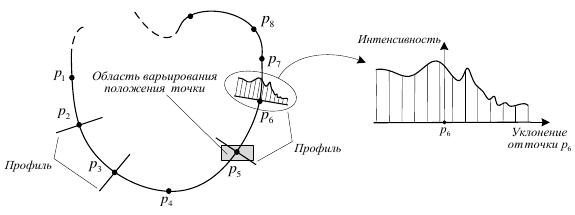
\includegraphics{contur.png}
    \caption{Профили точек контура}
    \label{fig:contur}
\end{figure}

Учитывая дискретность цифровых изображений, длина 
профиля измеряется в количестве пикселей. В аналогичных методах \cite{milborrow} длина профиля составляет 11-13 пикселей. При этом 
профиль описывается в виде вектора признаков. Характеристики \ref{math:imgs_classes} и \ref{math:kova_marks} рассматриваются как
статистическая модель, лежащая в основе оптимизации положения точек. 

Варьирование положения точек производится до тех пор, 
пока изменения существенно влияют на изменение формы контура. Оптимальным положением точки 
$p_k$ является такое, при 
котором профиль точки наименее отличается от усредненного 
профиля $q_k$.
Для определения степени сходства двух профилей 
применяется расстояние Махаланобиса, которое учитывает корреляцию между переменными и инвариантно к масштабу. 
Найденный в результате вариации точек контур может быть 
плохо согласован с совокупностью контуров обучающей выборки $\Im$ (рис. \ref{fig:crazy_face}).

\begin{figure}[hbt!]
    \centering
    \captionsetup{justification=centering}
    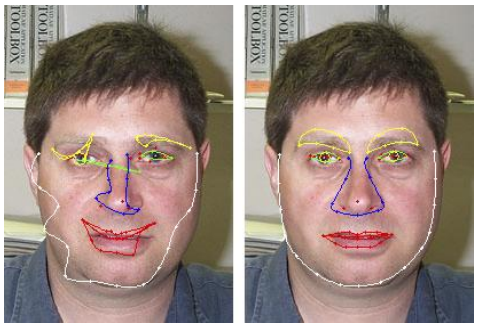
\includegraphics{crazy_face.png}
    \caption{Профильная оптимизация без сглаживания контура 
    (слева) и с применением сглаживания (справа)}
    \label{fig:crazy_face}
\end{figure}

Поэтому необходимо провести общую оптимизацию положения точек. Это достигается применением метода главных 
компонент. На этапе обучения вычисляются собственные значения ковариационной матрицы и матрица $\Phi$ соответствующих 
им собственных векторов. Вместо найденного контура $\mathit{X}$ рассматривается контур $\mathit{\widetilde{X}}$,
который вычисляется по контуру среднего лица $\overline{\mathit{X}}$ и матрице $\Phi$ собственных векторов:
$$\mathit{\widetilde{X}} = \overline{X} + \Phi\widetilde{b}.$$
Здесь $\widetilde{b}$~-- <<корректирующий>> вектор, который получается из вектора
коэффициентов проекции $b = \Phi^T(\mathit{X} - \overline{\mathit{X}})$ следующим образом:
\begin{enumerate}
    \item Обнуляются несущественные элементы вектора $b$ (соответствующие наименьшим по модулю собственным 
        значениям);
    \item Ненулевые элементы вектора 
        $b$ изменяются так, чтобы 
        гарантировать получение контура, лежащего внутри эллипсоида рассеяния. 
\end{enumerate}

\textit{Модель активных контуров является неустойчивой в следующих ситуациях:}
\begin{itemize}
    \item яркость рассматриваемого изображения значительно 
        отличается от яркости изображений, использованных 
        при построении модели; 
    \item низкая контрастность рассматриваемого изображения;
    \item плохая визуальная отделимость лица от фона изображения;
    \item отклонение ориентации лица от фронтального более чем на $10^{\circ}$;
    \item наличие предметов, закрывающих часть лица (головной убор, очки и др.).
\end{itemize}

Эксперименты показывают, что классификация 
при помощи СК не уступает современным аналогам при небольших объемах статистических выборок, а при увеличении 
объема выборки демонстрирует более высокое качество.

\subsubsection{Корреляционные методы обнаружения лиц}

Методы сопоставления по эталонам широкого используются для локации лиц на входных изображениях. При использовании этой методики
первоначально лица (в основном, изображения в анфас) предварительно детектируются и сохраняются в базе данных. Позже, вычисляется
корреляция между блоками вводимого изображения и сохраненными ранее эталонами. Преимуществами этого метода является его малая
чувствительность к шумам, простота в использовании и он не требует длительного времени для локации лица из вводимых изображений.

Однако, этого недостаточно для детекции лиц на изображениях с сильными вариациями фона и освещения, так как эти изменения могут
менять характерные формы распознаваемых объектов. Наиболее простой метод сопоставления по эталонам заключается в создании
усредненного эталона из набора изображений, хранящихся в базе данных (рис \ref{fig:average_persons}). В результате, прямоугольные блоки на входном изображении,
обладающие высокой корреляционной схожестью, предлагаются в качестве определения месторасположения лица. Такой метод можно назвать
техникой фильтруемого сопоставления с усредненным лицом в качестве фильтра\cite{correlations}.

\begin{figure}[hbt!]
    \centering
    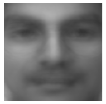
\includegraphics{average_persons.png}
    \caption{Усредненный эталон всех изображений}
    \label{fig:average_persons}
\end{figure}

Одним из широко используемых способов вычисления корреляции между усредненным эталоном лица и прямоугольными блоками входных
изображений является методика измерения схожести\cite{kvantic}. Некоторые функции для вычисления схожести данного изображения
с эталоном, представлены в таблице \ref{tables:correlations}.

Однако, на эти функции оказывают высокое влияние показатели освещенности и фоновые отражения т.к. на изображениях часто
встречаются блоки, не являющиеся частью лица, которые имеют те же параметры, что и матрица-эталон усредненного лица. Эта проблема
может быть решена с помощью алгоритма суммы абсолютных разностей (САР) \cite{sar}, который часто используется для сжатия изображений и
отслеживания объектов, но САР все же требует дополнительной оптимизации для вычисления более точного расположения лица на
изображении. Более того, САР может дать высокую точность локализации лица на изображении с высокой освещенностью, но помехи фона
могут повлиять на показатель точности. 

\begin{table}[bth]
    \centering
    \begin{tabu}{|X[c]|X[c]|}
        \hline
        Алгоритм & Вероятность верного обнаружения, \% \\
        \hline
        SAD & 94 \\
        \hline
        ZSAD & 94 \\
        \hline
        LSAD & 94 \\
        \hline
        SSD & 89 \\
        \hline
        LSSD & 89 \\
        \hline
        NCC & 73 \\
        \hline
        SHD & 40 \\
        \hline
    \end{tabu}
    \captionsetup{justification=centering}
    \caption{Сравнение корреляционных алгоритмов обнаружения лиц на фотоснимке}
    \label{tables:corr_results}
\end{table}

\begin{table}[hbtp]
    \begin{tabu}[\textwidth]{|X[c,2,m]||X[c,4,m]|}
        \hline
        Наименование & Формула \\
        \hline
        Сумма модулей разностей (Sum of Absolute Differences, SAD) &
        $$
        \sum_{(i,j)\in W} \vert I_1(i,j) - I_2(x + i, y + j)\vert
        $$
        \\\hline
        Сумма модулей разностей с нулевым средним значением (Zero-mean 
        Sum of Absolute Differences, ZSAD) &
        $$
        \sum_{(i,j)\in W} \vert I_1(i,j) - \overline{I}_1(i,j) - I_2(x + i, y + j) + \overline{I}_2(x+i, y+j) \vert
        $$
        \\\hline
        Локально взвешенная сумма модулей разностей (Locally scaled Sum 
        of Absolute Differences, LSAD) &
        $$
        \sum_{(i,j)\in W} \vert I_1(i,j) - \frac{\overline{I}_1(i,j)}{\overline{I}_2(x+i,y+j)}I_2(x+i,y+j)\vert
        $$
        \\\hline
        Сумма квадратов разностей (Sum of Squared Differences, SSD) &
        $$
        \sum_{(i,j)\in W} (I_1(i,j) - I_2(x + i, y + j))^2
        $$
        \\\hline
        Сумма квадратов разностей с нулевым средним значением (Zero-mean 
        Sum of Squared Differences, ZSSD) &
        $$
        \sum_{(i,j)\in W}(I_1(i,j) - \overline{I}_1(i,j) - I_2(x + i, y + j) + \overline{I}_2(x+i, y+j))^2
        $$
        \\\hline
        Локально взвешенная сумма квадратов разностей (Locally scaled Sum 
        of Squared Differences, LSSD) &
        $$
        \sum_{(i,j)\in W} (I_1(i,j) - \frac{\overline{I}_1(i,j)}{\overline{I}_2(x+i,y+j)}I_2(x+i,y+j))^2
        $$
        \\\hline
        Нормированная кросс корреляция (Normalized Cross Correlation, NCC) &
        $$
        \frac{\sum_{(i,j)\in W}I_1(i,j)I_2(x + i, y + j)}{\sqrt{\sum_{(i,j)\in W}(I_1(i,j) -
        \overline{I}_1(i,j))^2 I_{2_\Sigma}}},$$$$
        I_{2_\Sigma} = \sum_{(i,j)\in
        W}(I_2(x + i, y + j) - \overline{I}_2(x+i, y+j))^2
        $$
        \\\hline
        Сумма Хемминговых расстояний (Sum of Hamming Distances, SHD) &
        $$
        \sum_{(i,j)\in W}(I_1(i,j)\ \mathit{XOR}\ I_2(x + i, y + j))
        $$
        \\\hline
    \end{tabu}
    \captionsetup{justification=centering}
    \caption{Основные меры сходства двух изображений на основе кросс-корреляции}
    \label{tables:correlations}
\end{table}

Результаты обнаружения напрямую зависят от выбранного корреляционного алгоритма. В таблице \ref{tables:corr_results} приведены
результаты обнаружения лиц на 100 изображениях для некоторых алгоритмов.

\subsubsection{Обнаружение лица на основе цвета}

Детектор цвета кожи, используя представление объектов в цвете, позволяет найти изображение человеческого лица на фотографии или в
видеопотоке. В случае использования цветовой модели HSB для качественного детектирования необходимо правильно подобрать параметры
цвета кожи. 

Серьезным недостатком данного подхода является высокая зависимость результов обнаружения от яркости и освещенности изображения.
Однако, алгоритмы показывают хорошие результаты на снимках низкого качества т.к. они не зависят от геометрии лица.

Пример обнаружения представлен на рисунке \ref{fig:colors}.

\begin{figure}[hbt!]
    \centering
    \parbox{6cm}{
        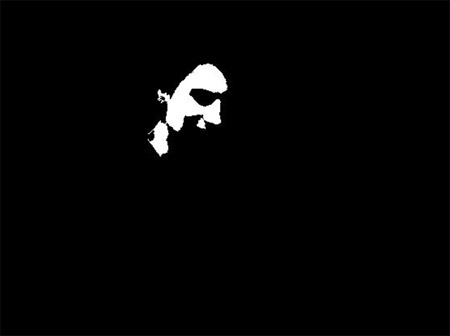
\includegraphics[width=6cm]{4.jpg}
    }\qquad
    \begin{minipage}{6cm}
        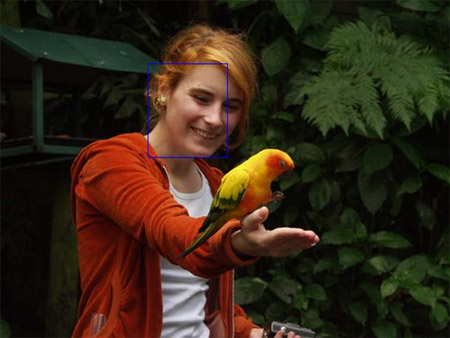
\includegraphics[width=6cm]{5.jpg}
    \end{minipage}
    \caption{Обнаружение лица на основе цвета}
    \label{fig:colors}
\end{figure}

\subsubsection{Алгоритм Виолы-Джонса}

Метод Виолы-Джонса \cite{viola_jones_2} является алгоритмом, основанным на антропологических особенностях лица~-- расположение
глаз, носа, рта и ушей. Метод является одним из лучших по соотношению показателей эффективность 
распознавания/скорость работы. Также этот детектор обладает низкой вероятностью ложного 
обнаружения лица. Алгоритм также хорошо работает и распознает черты лица под небольшим углом, 
примерно до 30 градусов, а так же при различных условиях освещенности.
Метод является основополагающим для поиска объектов на изображении в реальном времени и
реализован в таких проектах, как <<HxMarilena>>\cite{hxmerilena}, <<OpenClooVision>>\cite{cloovision}, <<MATLAB: Viola-Jones
Object Detection>>\cite{viola_matlab}, <<OpenCV>>\cite{opencv}, и других.

Алгоритм основан на использовании каскада признаков, которые называются \textit{примитивами Хаара}.
На рисунке \ref{fig:haar} изображены стандартные (слева) и дополнительные (справа) примитивы Хаара.

\begin{figure}[hbt!]
    \centering
    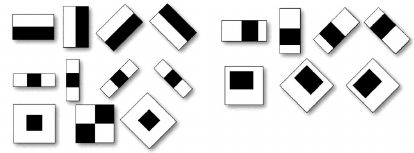
\includegraphics{haars.png}
    \caption{Примитивы Хаара}
    \label{fig:haar}
\end{figure}

Метод Виолы-Джонса в общем виде ищет лица и черты лица по общему принципу сканирующего окна, схема работы которого
представлена на рисунке \ref{fig:slide_win}.

\begin{figure}[hbt!]
    \centering
    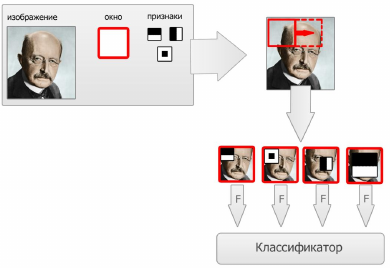
\includegraphics{slide_win.png}
    \caption{Схема работы принципа сканирующего окна}
    \label{fig:slide_win}
\end{figure}

Проверка прямоугольного признака на конкретной позиции проводится за константное время, что является преимуществом алгоритма по сравнению
с более точными методами. Каждая прямоугольная область в используемых признаках всегда смежна с другим прямоугольником, поэтому
расчет признака с 2 прямоугольниками состоит из 6 обращений в интегральный массив, для признака с 3 прямоугольниками -- из 8, с 4
прямоугольниками -- из 9.

Для выбора наиболее подходящих признаков для искомого объекта 
на части изображения используют алгоритм бустинга \cite{viola_jones_2}. Данный метод 
позволяет усилить простые классификаторы путём комбинирования 
примитивных <<слабых>> классификаторов в один <<сильный>>. Под <<силой>>
классификатора в данном случае подразумевается эффективность 
(качество) решения задачи классификации.

В работе алгоритм использует понятие \textit{интегрального изображения}.
В интегральном представлении изображений формируется матрица, совпадающая по размерам с
исходным изображением. В каждом ее элементе хранится сумма яркостей пикселей, находящихся левее и
выше данного элемента. Элементы матрицы рассчитываются по следующей формуле:
$$
    L(x, y) = \sum_{i = 0, j = 0}^{i \leq x, j \leq y}I(i,j)
$$

Где $I(i,j)$~-- яркость пикселя с координатой $(i, j)$.

Использование каскада Хаара имеет следующие плюсы:
\begin{itemize}
    \item описывают те знания о классе объектов, которые трудно 
        выделить на конкретном числе обучаемых данных;
    \item устойчивость к смене освещения, даже если это локальная 
        смена освещения, устойчивость к шумам (примитивы представляют собой 
        простейший полосовой фильтр);
    \item если примитивы были не очень маленькие, то сильно 
        устойчивее корреляции при изменении масштаба (размер примитивов при 
        этом не будет влиять на точность, если обход с маленьким шагом);
    \item если признаки на большом изображении рассчитать заранее и 
        при сдвиге окна поиска брать уже посчитанные и актуальные для него — 
        поиск будет значительно быстрее корреляции (нужно сравнить меньшее 
        количество элементов);
    \item такие системы работают гораздо быстрее, чем системы 
        работающие напрямую с пикселями. 
\end{itemize}

Обучение классификаторов идет очень медленно, но результаты поиска
лица очень быстры. Виола-Джонс является
одним из лучших по соотношению показателей эффективность
распознавания/скорость работы. Также этот детектор
обладает крайне низкой вероятностью ложного обнаружения лица. Алгоритм
даже хорошо работает и распознает черты
лица под небольшим углом, примерно до 30 градусов. При угле
наклона больше 30 градусов
процент обнаружений резко падает.

\subsection{Распознавание лиц}

Ключевым вопросом в анализе лиц
является представление данных о лице в виде, удобном для распознавания.
В начале 2000-х годов выделилось две базовые группы методов распознавания лиц:
холистические(глобальные) подходы и признаковые (структурные)
подходы. В первом случае, лица рассматриваются как цельные изображения,
которые сравниваются между собой. Во втором случае, из изображения лица
выделяются локальные признаки, такие как информация об абсолютном
и взаимном расположении глаз, носа, рта и т.п. Обе группы имеют свои
недостатки: холистические подходы показали в целом большую надежность
в близких к идеальным условиям распознавания по сравнению с признако-
выми подходами, однако признаковые подходы лучше себя зарекомендовали
в ситуации, когда отдельные части лица почему-либо не видны (например,
закрыты элементами одежды или очками).

Сначала будут рассмотрены методы из холистической группы: метод главных компонент,
линейный дискриминантный анализ, а затем методы из признаковой группы:
метод масштабно-инвариантного преобразования особенностей и метод
локальных бинарных шаблонов. Будут описаны их достоинства и недостатки,
а в конце раздела будет обоснован выбор метода, учитывая интересующие нас цели.

\subsubsection{Метод главных компонент}

Метод главных компонент (Principal Component Analysis - PCA)
\cite{PCA} является статистическим методом, уменьшающим размерность
данных. Используя изображение, как входные данные, метод не учитывает, что
объектом обработки являются изображения лиц. Он оперирует с векторами пикселей в
некотором линейном пространстве.


Опишем метод согласно \cite{volchenko}. $I$ --- черно-белое изображение лица
$Ver$ на $Hor$ пикселей, то есть
\[ I \in Mat(Ver \times Hor).\] $I \in \mathbb{R}^N$, где $N = Ver *
Hor$. Требуется определить некоторое подпространство $U \subset \mathbb{R}^N$,
размерности много меньшей N, при проекции на которое потеря информации
изображения $I \in \mathbb{R}^N$ будет минимальной.


Более подробно - пусть обучающая выборка лиц $\Omega = \{I_1,\dots,I_n\}, I_i
\in \mathbb{R}^N$. Математическое ожидание $E = E(\Omega) =
\frac{1}{n}\sum_{i=1}^nI_i$. Определим матрицу
\[ A =  [I_1 - E,\dots,I_n - E] \in Mat(N \times n),\]
и корреляционную матрицу
\[ C = \frac{1}{n}\sum_{i=1}^n(I_i - E)(I_i - E)^t = \frac{1}{n}AA^t \in Mat(N \times N). \]

Требуется найти правые собственные вектора матрицы C (они те же, что и у матрицы
D = nC). Это сложно сделать напрямую при больших значениях $N$, поэтому
используется другой путь.


Пусть $v$ - собственный вектор и $\lambda$ - соответствующее ему собственное
значение, тогда 
\[ Dv = \lambda v \Rightarrow AA^tv = \lambda v \Rightarrow A^tAA^tv = \lambda A^tv ,\]
следовательно, $y = A^tv$ - собственный вектор с собственным значением $\lambda$
для матрицы $A^tA \in Mat(n \times n)$, где n всего лишь число лиц в обучающей
выборке $\Omega$, а не размер изображения $N$.


Пусть $\{r_1,\dots,r_k\}$ - первые $k$ векторов $(k \leq n)$, отвечающих
наибольшим различным собственным значениям матрицы $A^tA$, то есть
\[ A^tAr_i = \lambda_ir_i \Rightarrow AA^tAr_i = \lambda_iAr_i \Leftrightarrow AA^tv_i = \lambda_iv_i \Leftrightarrow Dv_i = \lambda_iv_i,\]
где $v_i = Ar_i$. Следовательно, $v_i$ являются собственными векторами матрицы
$D$. Заметим, что каждый $v_i$ есть линейная комбинация векторов $I_1 -
E,\dots,I_n - E$, то есть линейная комбинация исходных лиц $I_1,\dots,I_n$. В
связи с чем, $v_i$ имею лицеподобный вид, их часто называют собственными лицами
(eigenfaces) \label{fig:pca-faces}.

\begin{figure}[h!]
  \centering
  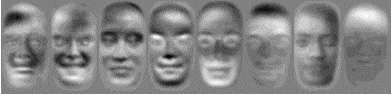
\includegraphics[width=0.7\textwidth]{pca_faces.png}
  \caption{Собственные лица}
  \label{fig:pca-faces}
\end{figure}

Произвольность обучающей выборки $\Omega$, как правило, позволяет считать, что
$rg(A) = n$ (то есть максимальный ранг) и все вектора $r_1,\dots,r_k$ ---
линейно независимы. Следовательно, вектора $v_i = Ar_i (i = 1,\dots,k)$ тоже
линейно независимы и образуют подпространство $U = Lin\langle
v_1,\dots,v_k\rangle$ размерности $k$. Более того, вектора $v_i$ -
ортогональны. В самом деле: так как $\lambda_i(v_i,v_j) = (AA^tv_i,v_j) =
(v_i,(AA^t)^tv_j) = (v_i, AA^tv_j) = \lambda_j(v_i,v_j)$, где $(\cdot,\cdot)$
--- скалярное произведение. В таком случае, если $\lambda_i \neq \lambda_j$, то
$(v_i,v_j) = 0$.


Любой вектор $I = (i_1,\dots,i_N)^t$ ортогонально проецируется в подпространство
$U$. $J = Pr_U(I) = (j_1,\dots,j_k)^t \in \mathbb{R}^k, j_i = (I,v_j)$. В силу
максимальности собственных значений, отвечающих $v_i$, набор чисел
$j_1,\dots,j_k$ характеризуют случайную величину $I$ по наиболее значимым
параметрам, и в силу ортогональности $v_i (i=1,\dots,k$, эти параметры
независимы. Теперь изображение любого лица представляется вектором в $k$-мерном
пространстве, где $k$ много меньше $N$.


Степень различия между двумя лицами определяется как $\rho(A,B) = \sum a_ib_i$,
где $A = (a_1,\dots,a_k), B = (b_1,\dots,b_k)$ - проекция изображений двух
лиц. Если два изображения похожи, то различие между их проекциями мало, поэтому,
изображения одного человека определяют некоторую область в $U$.


Для функционирования алгоритма распознавания требуется определить
подпространство $U$. При этом, $\Omega$ должна содержать по возможности
наибольшую выборку различных изображений лиц. Следует отметить, что все лица
должны быть в одном положении, например в фас, а также изображения должны быть
одинакового размера - $Ver$ на $Hor$ пикселей.


Пусть $\{\Omega_i, (i=1,\dots,K)\}$. $\Omega_i = \{I_1^i,\dots,I_{n(i)}^i\}$
множество изображений $i$-ого человека. Находим $\Lambda_i = Pr_U(\Omega_i) =
\{J_1^n,\dots,J_{n(i)}^i\}$, где $J_t^i = Pr_U(I_t^i - E)$. Если требуется
распознать неизвестное изображение $A$, то находим $B = Pr_U(A - E)$. Затем,
среди векторов $\{J_1^i,\dots,J_{n(i)}^i\} (i=1,\dots,K)$ находим $J_m^t$
ближайший к $B$. Если расстояние между $J_m^i$ и $B$ не превосходит некоторого
порогового значения $D_{min}$, то считаем, что вектор $B$ принадлежит классу
$t$, и $A$ - это изображение лица с номером $t$. Если расстояние между $J_m^i$ и
$B$ больше $D_{min}$, то считаем, что человека с изображением A нет. Пороговое
значение $D_{min}$ устанавливается эмпирически.


Эффективность распознавания зависит от размерности $U$, то есть от количества
собственных лиц, от качества изображений: разрешения, освещенности, расположения
лица на изображении, и т.д. Необходимо иметь одинаковое освещение и положение
головы на всех изображениях, хотя допустимы небольшие отклонения: очки, небольшие
повороты головы, улыбки и т.п.

Метод имеет следующие преимущества:
\begin{enumerate}
\item При наличии в наборе изображений лиц вариаций, таких как раса, пол,
эмоции, освещение, будут появляться компоненты, величина которых в основном
определяется этими факторами. Поэтому по значениям соответствующих главных
компонент можно определить, например, расу или пол человека;
\item Хранение и поиск изображений в больших базах данных, реконструкция
изображений.
\end{enumerate}

Метод имеет следующие недостатки:
\begin{enumerate}
\item Изображения должны быть получены в близких условиях освещённости,
одинаковом ракурсе;
\item Должна быть проведена качественная предварительная
обработка, приводящая изображения к стандартным условиям.
\end{enumerate}


\subsubsection{Линейный дискриминантный анализ}

Линейный дискриминантный анализ (ЛДА)~\cite{LDA}, а также связанный с ним
линейный дискриминант Фишера — методы статистики и машинного обучения,
применяемые для нахождения линейных комбинаций признаков, наилучшим образом
разделяющих два или более класса объектов или событий. Полученная комбинация
может быть использована в качестве линейного классификатора или для сокращения
размерности пространства признаков перед последующей классификацией. ЛДА тесно
связан с дисперсионным анализом и регрессионным анализом, также пытающимися
выразить какую-либо зависимую переменную через линейную комбинацию других
признаков или измерений. В этих двух методах зависимая переменная — численная
величина, а в ЛДА она является величиной номинальной (меткой класса). Помимо
того, ЛДА имеет схожие черты с методом главных компонент и факторным анализом,
которые ищут линейные комбинации величин, наилучшим образом описывающие
данные. Для использования ЛДА признаки должны быть непрерывными величинами,
иначе следует использовать анализ соответствий (англ. Discriminant Correspondece
Analysis).


Рассмотрим ЛДА в случае наличия двух классов. Для каждого образца объекта или
события с известным классом $y$ рассматривается набор наблюдений $x$ (называемых
ещё признаками, переменными или измерениями). Набор таких образцов называется
обучающей выборкой (или набором обучения, обучением). Задачи классификации
состоит в том, чтобы построить хороший прогноз класса $y$ для всякого так же
распределённого объекта (не обязательно содержащегося в обучающей выборке), имея
только наблюдения $x$.


При ЛДА предполагается, что функции совместной плотности распределения
вероятностей $p(\vec{x}|y=1)$ и $p(\vec{x}|y=0)$ - нормальны. В этих
предположениях оптимальное байесовске решение - относить точки ко второму классу
если отношение правдоподобия ниже некоторого порогового знчения $T$:
$$ (\vec{x}-\vec{\mu}_0)^T\Sigma_{y=0}^{-1}(\vec{x}-\vec{\mu}_0)+\ln{|\Sigma _{y=0}|}-(\vec{x}-\vec{\mu}_1)^T\Sigma_{y=1}^{-1}(\vec{x}-\vec{\mu}_1)\ln{|\Sigma_{y=0}|}<T $$


Если не делается никаких дальнейших предположений, полученную задачу
классификации называют квадратичным дискриминантным анализом (англ. quadratic
discriminant analysis, QDA). В ЛДА делается дополнительное предположение о
гомоскедастичности (т.е. предполагается, что ковариационные матрицы равны,
$\Sigma_{y=0}=\Sigma_{y=1}=\Sigma$) и считается, что ковариационные матрицы
имеют полный ранг. При этих предположениях задача упрощается и сводится к
сравнению скалярного произведения с пороговым значением
$$ \vec{\omega}\cdot\vec{x}<c $$
для некоторой константы $c$, где 
$$ \vec{\omega}=\Sigma^{-1}(\vec{\mu_1}-\vec{\mu_0}). $$
Это означает, что вероятность принадлежности нового наблюдения $x$ к классу $y$
зависит исключительно от линейной комбинации известных наблюдений.


Зачастую понятия линейный дискриминант Фишера и ЛДА используют в качестве
синонимов, хотя в исходной статье Рональда Эйлмера Фишера Использование
множественных мер в задачах таксономии (The use of multiple measurements in
taxonomic problems, 1936) описывается несколько иной дискриминант и не
принимаются некоторые характерные для ЛДА предположения, такие, как нормальность
распределений или равенство дисперсий.


Предположим, что два наблюдаемых класса имеют средние
$\vec{\mu}_{y=0},\vec{\mu}_{y=1}$ и ковариационные матрицы
$\Sigma_{y=0},\Sigma_{y=1}$. Тогда для линейной комбинации признаков
$\vec{\omega}\cdot\vec{x}$ средними будут $\vec{\omega}\cdot\vec{\mu_{y=i}}$, а
ковариационные матрицы будут иметь вид $\vec{\omega}^T\Sigma_{y=i}\vec{\omega}$
для $i=0,1$. Фишер взял за расстояние между этими распределениями величину,
равную отношению межклассовой дисперсии к внутриклассовой:
$$S=\frac{\sigma^2_{between}}{\sigma^2_{within}}=\frac{(\vec{\omega}\cdot\vec{\mu}_{y=1}-\vec{\omega}\cdot\vec{\mu}_{y=0})^2}{\vec{\omega}^T\Sigma_{y=1}\vec{\omega}+\vec{\omega}^T\Sigma_{y=0}\vec{\omega}}=\frac{(\vec{\omega}\cdot(\vec{\mu}_{y=1}-\vec{\mu}_{y=0}))^2}{\vec{\omega}^T(\Sigma_{y=1}+\Sigma_{y=0})\vec{\omega}}
$$

Эта величина в некотором смысле характерезует соотношение сигнал-шум для
разметки классов. Можно показать, что наилучшим образом классы разделимы при
$$ \vec{\omega}=(\Sigma_{y=1}+\Sigma_{y=0})^{-1}(\vec{\mu}_{y=1}-\vec{\mu}_{y=0}). $$

Если выполняются предположения нормальности и равенства дисперсий, то полученное
выше равенство эквивалентно ЛДА. Обратим внимание, что вектор $\vec{\omega}$
является вектором нормали к разделяющей гиперплоскости. Например в двумерном
случае линия, наилучшим образом разделяющая два класса, перпендикулярна к
$\vec{\omega}$. В общем случае строятся проекции точек (образов данных в
пространстве признаков) на $\vec{\omega}$. Однако, чтобы в точности найти
оптимально разделяющую данные гиперплоскость, требуется найти влияющую на её
положение величину b из уравнения
$\vec{\omega}^T\mu_0+b=-(\vec{\omega}^T\mu_1+b)$.


Рассмотрим ЛДА в случае, когда количество классов больше двух. В случае, когда
классов больше двух, рассуждения, использованные при выведении линейного
дискриминанта Фишера, могут быть дополнены для поиска подпространства,
содержащего все объекты класса. Предположим, что каждый из $C$ классов имеет
среднее $\mu_i$ и одну и ту же ковариационную матрицу $\Sigma$. Тогда
межклассовое рассеяние может быть задано, как ковариация средних:
$$ \Sigma_b=\frac{1}{C}\sum_{i=1}^C (\mu_i-\mu)(\mu_i-\mu)^T, $$
где $\mu$ — среднее по всем классам. Расстояние между классами в направлении
$\vec{\omega}$ в этом случае:
$$
 S=\frac{\vec{\omega}^T\Sigma_b\vec{\omega}}{\vec{\omega}^T\Sigma\vec{\omega}}=\frac{\vec{\omega}^T(\Sigma_b\Sigma^{-1})\Sigma\vec{\omega}}{\vec{\omega}^T\Sigma\vec{\omega}}.
 $$


Это означает, что, когда $\vec{\omega}$ — собственный вектор матрицы
$\Sigma_b\Sigma^{-1}$, расстояние будет равно соответствующему собственному
значению. Т.к. ранг $\Sigma_b$ не превосходит $C-1$, эти ненулевые собственные
векторы задают искомое векторное подпространство. Основное применение этих
векторов - генерация признаков, как, например, в методе главных компонент.


На практике средние классов и ковариации неизвестны. Их, однако, можно оценить,
основываясь на данных обучения. В описанных выше равенствах можно вместо точных
значений использовать апостериорные оценки или оценки максимального
правдоподобия. Но, хотя в некотором смысле оценка ковариаций может считаться
оптимальной, полученная после замены точных данных оценками разделяющая
гиперплоскость не обязательно будет оптимальной, даже при верности предположения
о нормальности распределений.


Другая сложность, возникающая при практическом использовании ЛДА и линейного
дискриминанта Фишера, возникает, если в обучающихся данных многократно
встречаются одинаковые объекты (число наблюдений каждого объекта превышает
суммарное количество объектов). В этом случае оценки для матриц ковариаций имеют
неполный ранг и поэтому не могут быть обращены. Существует несколько путей
борьбы с этой проблемой. Один из них — использовать псевдообращение, вместо
обычного обращения ковариационных матриц. Другой, называемый регуляризованным
дискриминантным анализом, заключается в искусственном увеличении числа доступных
объектов обучения за счёт добавления белых шумов. Эти новые объекты обучения не
обязательно просчитывать, т.к. их влияние на ковариации классов можно выразить
как:
$$ C_{new}=C+\sigma^2I, $$
где $I$ --- единичная матрица, а величина $\sigma$, называемая в данном случае
регуляризующим параметром, --- количество добавленных шумов. Значение $\sigma$
обычно определяют методом скользящего контроля. Новая ковариационная матрица
всегда обратима и может быть использована в вычислениях.


ЛДА может быть обобщён на случай множественного дискриминантного анализа, где c
становится качественной переменной с $N$ возможными значениями вместо двух. Если
условные плотности распределения $p(\vec{x}|c=i)$ нормальны и матрицы ковариации
одинаковы, достаточной статистикой для $P(c|\vec{x})$ будут значения $N$
проекций, образующих подпространство, натянутое на $N$ средних и афинно
спроектированное с помощью обратной ковариацонной матрицы. Эти проекции могут
быть найдены, решая обобщённую задачу на собственные значения, где в качестве
числителя выступает ковариационная матрица, получающаяся при рассмотрении в
векторов средних качестве образцов, а в качестве знаменателя — общая
ковариационная матрица.


На компьютере распознаваемое лицо представлено в виде большого количества
значений-пикселей. ЛДА используется для сокращения перед классификацией
количества признаков до количества, более удобного в работе. Каждая новая
размерность является линейной комбинацией значений пикселей, которые формируют
темплэйты (от англ. template —- шаблон). Линейные комбинации, полученные с
помощью линейного дискриминанта Фишера, называют фишеровскими лицами, а
полученные с помощью схожего метода главных компонент, — собственными лицами.

Метод имеет следующие преимущества:
\begin{enumerate}
\item Высокая точность распознавания (около 94\%);
\item Высокие показатели распознавания при широком диапазоне условий 
освещённости, различных выражениях лица и наличии или отсутствии очков.
\end{enumerate}

Метод имеет следующие недостатки:
\begin{enumerate}
\item Открытые вопросы о том, применим ли этот метод для поиска в
больших базах данных, может ли метод работать, когда в тренировочной выборке для
некоторых лиц имеется изображение только в одних условиях освещённости;
\item Необходимость в предварительной обработке;
\item Плохие показатели распознавания при изменении ракурса.
\end{enumerate}



\subsubsection{Масштабно-инвариантное преобразование особеностей}

Метод масштабно-инвариантного преобразования особенностей (SIFT --- Scale
In\-va\-ri\-ant Feature Transformation) позволяет извлечь из изображений особенности
для сопоставления различных поз одного и того же объекта. Метод нечувствителен
к масштабу и ориентации.


Сначала нужно найти особые точки. Основным моментом в детектировании особых
точек является построение пирамиды гауссианов (Gaussian) и разностей гауссианов
(Difference of Gaussian, DoG). Гауссианом (или изображением, размытым гауссовым
фильтром) является изображение
$$ L(x,y,\sigma) = G(x,y,\sigma) \ast I(x,y), $$
где $L$ --- значение гауссиана в точке с координатами $(x,y)$, а $\sigma$ ---
радиус размытия. $G$ - гауссово ядро, $I$ --- значение исходного изображения,
$\ast$ --- операция свертки.


Разностью гауссианов называют изображение, полученное путем попиксельного
вычитания одного гауссиана исходного изображения из гауссиана с другим радиусом
размытия.
$$ D(x,y,\sigma) = (G(x,y,k\sigma) - G(x,y,\sigma)) \ast I(x,y) = L(x,y,k\sigma) - L(x,y,\sigma). $$


Инвариантность относительно масштаба достигается за счет нахождения ключевых
точек для исходного изображения, взятого в разных масштабах. Для этого строится
пирамида гауссианов: все масштабируемое пространство разбивается на некоторые
участки — октавы, причем часть масштабируемого пространства, занимаемого
следующей октавой, в два раза больше части, занимаемой предыдущей. К тому же,
при переходе от одной октавы к другой делается ресэмплинг изображения, его
размеры уменьшаются вдвое. Естественно, что каждая октава охватывает бесконечное
множество гауссианов изображения, поэтому строится только некоторое их
количество $N$, с определенным шагом по радиусу размытия. С тем же шагом
достраиваются два дополнительных гауссиана (всего получается $N+2$), выходящие
за пределы октавы. Далее будет видно, зачем это нужно. Масштаб первого
изображения следующей октавы равен масштабу изображения из предыдущей октавы с
номером $N$.


Параллельно с построением пирамиды гауссианов, строится пирамида разностей
гауссианов, состоящая из разностей соседних изображений в пирамиде
гауссианов. Соответственно, количество изображений в этой пирамиде будет $N+1$.


Будем считать точку особой, если она является локальным экстремумом разности
гауссианов. Для поиска экстремумов будем использовать метод, схематично
изображенный на рисунке \ref{fig:sift-extr}.

\begin{figure}[h!]
  \centering
  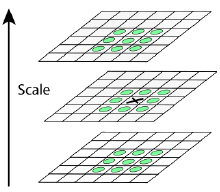
\includegraphics[height=.2\textheight]{sift-extremum.png}
  \caption{Метод поиска экстремумов.}
  \label{fig:sift-extr} 
\end{figure}

В каждом изображении из пирамиды DoG ищутся точки локального экстремума. Каждая
точка текущего изображения DoG сравнивается с её восьмью соседями и с девятью
соседями в DoG, находящихся на уровень выше и ниже в пирамиде. Если эта точка
больше (меньше) всех соседей, то она принимается за точку локального экстремума.


Для того, чтобы проверить на наличие точек экстремума $N$'e изображение в DoG
пирамиде, нужно иметь $N+1$'е. А для того, чтобы получить $N+1$'е в DoG
пирамиде, надо иметь $N+1$'е и $N+2$'е изображения в пирамиде гауссианов. Следуя
той же логике можно сказать, что нужно строить 0'е изображение (для проверки
1'го) в пирамиде DoG и ещё два в пирамиде гауссианов. Но 1'е изображение в
текущей октаве имеет тот же масштаб, что и $N$'е в предыдущей (которое уже
должно быть проверено).


Рассмотрим уточнение особых точек. Проверяем пригодность точки экстремума на
роль ключевой.


Определяются координаты особой точки с субпиксельной точностью. Это достигается
с помощью аппроксимирования функции DoG многочленом Тейлора второго порядка,
взятого в точке вычисленного экстремума.
$$ D(x) = D + \frac{\partial D^T}{\partial x}x + \frac{1}{2}x^T\frac{\partial^2D}{\partial x^2}x, $$
где $D$ - функция DoG, $X = (x,y,\sigma)$ --- вектор смещения относительно точки
разложения, первая производная DoG --- градиент, вторая --- матрица Гессе.


Экстремум многочлена Тейлора находится путем вычисления производной и
приравнивания ее к нулю. В итоге получим смещение точки вычисленного экстремума,
относительно точного
$$ \widehat{x} = -\frac{\partial^2D^{-1}}{\partial x^2}\frac{\partial D}{\partial x}. $$

Все производные вычисляются по формулам конечных разностей. В итоге получаем
СЛАУ размерности $3 \times 3$, относительно компонент вектора $\widehat{x}$.


Если одна из компонент вектора $\widehat{x}$ больше половины шага сетки в этом
направлении, то это означает, что на самом деле точка экстремума была вычислена
неверно и нужно сдвинуться к соседней точке в направлении указанных
компонент. Для соседней точки все повторяется заново. Если таким образом мы
вышли за пределы октавы, то следует исключить данную точку из рассмотрения.


Когда положение точки экстремума вычислено, проверяется на малость само значение
DoG в этой точке по формуле
$$ D(\widehat{x}) = D + \frac{1}{2}\frac{\partial D^T}{\partial x}\widehat{x}. $$

Если последняя проверка не проходит, то точка исключается, как точка с малым
контрастом.


Строим гистограмму ориентаций $\theta(x,y)$
$$m(x,y) = \sqrt{((L(x+1),y) - L(x-1,y))^2 + (L(x,y+1)-L(x,y-1))^2}, $$
$$\theta(x,y) = tanh(L(x,y+1) - L(x,y-1) / (L(x+1,y) - L(x-1,y)). $$

Вычисляем дескрипторы ключевых точек. Далее дескриптор локальных
особенностей вычисляется для каждой ключевой точки. Он основан на локальном
градиенте изображения, трансформированном в соответствии с ориентацией ключевой
точки, чтобы предоставить неизменность ориентации. Каждая особенность --- это
вектор с размерностью 128 явно идентифицирующий окрестности ключевой точки.


Дескриптор каждой ключевой точки, вычисленной для нового изображения лица,
независимо сравнивается с сохраненными дескрипторами ключевых точек лиц, и при
достаточном совпадении считаем, что лица совпадают.

Метод имеет следующие преимущества:
\begin{enumerate}
\item Более высокие показатели распознавания по сравнению с холистическими
методами (PCA, LDA);
\item Инвариантность метода к масштабу.
\end{enumerate}

Метод имеет следующие недостатки:
\begin{enumerate}
\item На лице человека обычно слишком мало углов, для которых определяются
ключевые точки;
\item Запатентован в США, что делает невозможным коммерческое использования без
получения разрешения автора.
\end{enumerate}

\subsubsection{Метод локальных бинарных шаблонов}

Изначально оператор LBP \cite{LBP} был создан для описания текстуры. Оператор
сопоставляет каждому пикселю 8-битное значение, вычисляемое в зависимости от
значений интенсивностей рассматриваемого пикселя и его 8-ми соседей, как
показано на рисунке \ref{fig:lbp-operator}. Затем гистограммы таких значений
различных регионов лица могут быть использованы в качестве дескриптора текстуры
лица.


Локальные бинарные шаблоны вычисляются путем применения определенного оператора
к каждому пикселю изображения. Этот оператор работает следующим образом. Вначале
значение интенсивности в пикселе сравнивается со значениями во всех пикселях из
некоторой окрестности, например, размером $3\times3$ пикселя. Результат сравнения
записывается как 0, если значение рассматриваемого пикселя меньше центрального,
и как 1 в противном случае. Для рассматриваемой окрестности 3 на 3 получается 8
цифр, из которых составляется двоичный вектор, который интерпретируется как
двоичная запись целого числа. Это число и является результатом применения
оператора к пикселю. Итоговые признаки получаются после разбиения всего
изображения решеткой на прямоугольные области, подсчета гистограмм частот
появления чисел в каждой области и конкатенации гистограмм по всем областям в
один вектор. Процесс вычисления локальных бинарных шаблонов показан на рисунке
\ref{fig:lbp-operator}.

\begin{figure}[h!]  \centering
  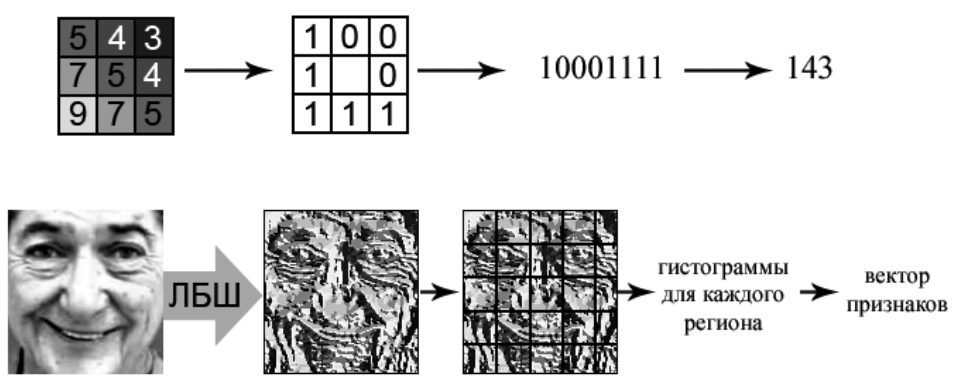
\includegraphics[height=.2\textheight]{lbp-operator.png}
    \captionsetup{justification=centering}
  \caption{Вычисление локальных бинарных шаблонов: вверху – для одного пикселя,
внизу – для целого изображения.}
  \label{fig:lbp-operator}
\end{figure}

Признаки, полученные таким образом, устойчивы к небольшим изменениям
освещенности и небольшим сдвигам в положении лица \ref{fig:lbp-faces}. Эта
устойчивость достигается за счет того, что подсчет ведется не индивидуально для
каждого пикселя, а используются области значительного размера.

\begin{figure}[h!]  \centering
  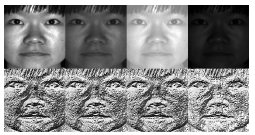
\includegraphics[height=.2\textheight]{lbp-faces.png}
    \captionsetup{justification=centering}
  \caption{Пример использования оператора lbp для изображений лиц с различной
степенью освещенности.}
  \label{fig:lbp-faces}
\end{figure}

Более формально оператор LBP можно описать так:
\[ LBP(x_C,y_c) = \sum_{p=0}^{p-1}2^ps(i_p-i_c),\] где $(x_c,y_c)$ ---
координаты центрального пикселя с интесивностью $i_c$; $i_n$ --- интенсивность
соседнего пикселя, а s --- функция, определенная следующим образом:
\[ s(x) = \begin{cases} 1, \mbox{если $x \geq 0$} \\ 0, \mbox{иначе}
          \end{cases}
\]

В скором времени было обнаружено, что данный оператор не может закодировать
детали в различном масштабе. Тогда данный оператор был расширен, чтобы
использовать произвольные соседние пиксели. Идея заключается в том, чтобы задать
радиус отступа от рассматриваемого до интересующих нас пикселей и количество
пикселей-соседей. Для рассматриваемой точки $(x_p,y_p)$ позиция соседа
$(x_p,y_p),p \in P$ может быть вычислена так:
\[ x_p = x_c + R\cos(\frac{2\pi p}{P}) \]
\[ y_p = y_c - R\sin(\frac{2\pi p}{P}), \] где R --- радиус
окружности(расстояние от рассматриваемого пикселя до соседей), а P ---
количество рассматриваемых соседей.


Такой оператор является расширением оригинального LBP, так что он называется
расширенным LBP (Extended LBP) либо круговым LBP (Circular LBP). Если координата
точки на окружности не совпадает с координатой на изображении, можно получить
координаты точки с помощью интерполяции. Например, билинейной:
$$ f(x,y) \approx 
\begin{bmatrix} 1 - x & x
\end{bmatrix}
\begin{bmatrix} f(0,0) & f(0,1) \\ f(1,0) & f(1,1)
\end{bmatrix}
\begin{bmatrix} 1 - y \\ y
\end{bmatrix}
$$


Из рисунка \ref{fig:lbp-operator} можно увидеть, что процесс выделения признаков
из изображения с помощью оператора LBP состоит из следующих шагов:
\begin{enumerate}
\item Выбрать количество регионов, на которые будем делить изображение;
\item Выбрать радиус окружности и количество точек, участвующих в рассмотрении,
если используется оператор Расширенный LBP;
\item Разделить изображение, посчитать гистограммы количества одинаковых
значений оператора, примененного для каждого пикселя области, для каждой
области;
\item Соединить их в результирующий вектор, который и будет представлять наше
изображение.
\end{enumerate}


\subsubsection{Вайвлет-преобразование}

Вейвлет-преобразование широко используется
для анализа нестационарных процессов. Оно показало свою эффективность для решения широкого
класса задач, связанных с обработкой изображения. Коэффициенты вейвлет-преобразования со
держат информацию об анализируемом процессе
и используемом вейвлете. Поэтому выбор анализирующего вейвлета определяется тем, какую информацию необходимо извлечь из процесса. Каждый
вейвлет имеет характерные особенности во временной и частотной областях, поэтому иногда
с помощью разных вейвлетов можно полнее выявить и подчеркнуть те или иные свойства анализируемого процесса.

В работах \cite{vaivlet_1,vaivlet_2} представлены разложение изображения и извлечение его признаков для классификации изображений
самолетов на основе применения вейвлетпреобразования Хаара и многослойной нейронной сети. В данной работе используются вейвлет-преобразования Хаара и Добеши
для извлечения признаков изображения лиц. Примеры применения вейвлетпреобразования Хаара
и вейвлетпреобразования Добеши для извлечения
признаков изображения лица представлены на
рисунке \ref{fig:dobeshi_haar}.

\begin{figure}[hbt!]
    \centering
    \parbox{6cm}{
        \centering
        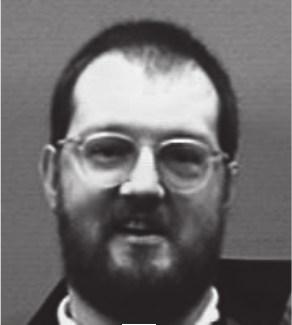
\includegraphics[height=5cm]{debosh_haar.png}
        \caption*{б}
    }\qquad
    \begin{minipage}{6cm}
        \centering
        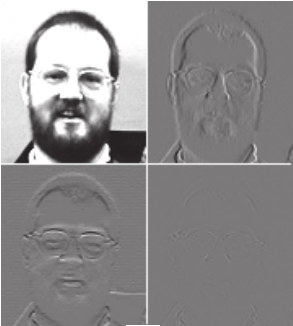
\includegraphics[height=5cm]{debosh_haar_2.png}
        \caption*{а}
    \end{minipage}
    \captionsetup{justification=centering}
    \caption{Пример извлечения признаков лица: а)~исходное изображение лица; б)~результат применения вайвлет-преобразования Хаара.}
    \label{fig:dobeshi_haar}
\end{figure}

Согласно \cite{vaivlet_1} выведем математические выражения, описывающие Вайвлет-преобра\-зование Добеши.
Преобразование будет применяться к последовательности из четырех точек с шагом в две точки.

Результат преобразования будет состоять из двух последовательностей: результата высокочастотной фильтрации и результата
низкочастотной фильтрации.

Рассмотрим последовательность яркостей $ (x,y,z,t) $. В этом случае первый фильтр запишем в виде:

\begin{equation}
    a = c_1x + c_2y + c_3z + c_4t
    \label{eq:high_filter}
\end{equation}

Четыре коэффициента, образующих вектор-строку матрицы преобразования, пока неизвестны.
Вектор-строка коэффициентов второго фильтра ортогональна строке коэффициентов первого фильтра.
Поэтому, перепишем уравнение \ref{eq:high_filter} для низкочастотного фильтра:

$$
    d = c_4x - c_3y + c_2z - c_1t
$$

Матрица преобразования будет иметь вид:
$$
\begin{pmatrix}c_1 & c_2 & c_3 & c_4 & & & \\
c_4 & -c_3 & c_2 & c_1 & & & \\
& & c_1 & c_2 & c_3 & c_4 & \\
& & c_4 & -c_3 & c_2 & c_1 & \\
&&&&&& \ddots \end{pmatrix}
$$

Требование ортогональности выполняется для первой и второй строк автоматически. Потребуем, чтобы строки 1 и 3 тоже были
ортогональны:
$$
c_3c_1+c_4c_2=0
$$

Векторы должны иметь единичную длину (иначе определитель будет не единичным):
$$
c_1^2 + c_2^2+c_3^2+c_4^2 = 1
$$

Преобразование должно обнулять цепочку одинаковых значений (например, $(1, 1, 1, 1)$):
$$
    1c_1+1c_2+1c_3+1c_4=0
$$

Преобразование должно обнулять цепочку линейно растущих значений (например, $(1, 2, 3, 4)$):
$$
    1c_4-2c_3+3c_2-4c_1=0
$$

Получили 4 уравнения, связывающие коэффициенты. Решая их, получаем:
$$
    c_1=\frac{1+\sqrt{3}}{4\sqrt{2}};\ 
    c_2=\frac{3+\sqrt{3}}{4\sqrt{2}};\ 
    c_3=\frac{3-\sqrt{3}}{4\sqrt{2}};\ 
    c_4=\frac{1-\sqrt{3}}{4\sqrt{2}}.
$$

Подставив их в матрицу, получаем искомое преобразования.
Это преобразование получило название вейвлета D4\cite{vaivlet_1}.
Чтобы выполнить двумерное преобразование Добеши (или аналогичное ему), нужно лишь выполнить его для каждой строки и для каждого
столбца.

Результат двумерного преобразования позволяет выделить скачки интенсивности цвета,
что в результате выявляет и подчеркивает особенности каждого изображения.

Преимуществами данного метода является очень высокая производительность, простота вычислений и независимость
от условий освещенности.
Однако фильтр чувствителен к изменению ракурса съемки.

\subsection{Классификация}

Классификацию предполагается производить с помощью нейронной сети,
обучаемой методом обратного распространения ошибки, так как данный метод
классификации предоставляет широкий спектр настроек (подбор коэффициентов) и
делает возможным последующие улучшения, например построение сети глубокой
архитектуры.

\subsection{Существующие методы и программные продукты}

Проблема распознавания лиц рассматривалась еще на ранних
стадиях компьютерного зрения. Поэтому
существует множество методов для обнаружения и распознавания человеческого
лица по фотоснимку.
Ряд компаний на протяжении более 40 лет активно разрабатывают
автоматизированные, а сейчас и автоматические системы распознавания
человеческих лиц, например 
ImageWare (система FaceID \cite{faceid}) и Imagis Technologies Inc. (система
ID-2000 Image Detection and Biometric Facial Recognition \cite{imagis}).

Основными характеристиками, которыми различаются указанные системы, являются:
\begin{itemize}
    \item возможность поиска и распознавания нескольких лиц;
    \item устойчивость к изменениям в прическе, наличию/отсутствию усов
        и бороды, очкам (кроме солнцезащитных), возрастным
        изменениям (кроме детей), поворотам (до и более 30 градусов)
    \item возможность многокадрового анализа видеопотока,
        обеспечивающего повышение точности распознавания;
    \item слабая зависимость скорости работы от размера используемой
        галереи лиц. Например, при увеличении галереи со 100 до
        1000 лиц, скорость работы уменьшается менее чем на 10\%;
    \item работа с видео в режиме реального времени.
\end{itemize}

Указанные системы являются закрытыми для рядового пользователя и разработчика.
Однако существует и набор программных продуктов, распространяющихся по
открытой лицензии BSD, среди которых находится система OpenCV~\cite{opencv}.

OpenCV~-- библиотека компьютерного зрения с открытым исходным кодом
(Open Source Computer Vision Library), содержащая более 500
функций, заточенных под выполнение в реальном времени.

Библиотека содержит алгоритмы для обработки, реконструкции и
очистки изображений, распознания образов, захвата видео,
слежения за объектами, калибровки камер и др.

Открытая лицензия для OpenCV была составлена таким образом, чтобы было
возможно создавать коммерческие приложения, используя
любые возможности OpenCV. 
Отчасти из-за таких условий существует
большое сообщество пользователей, включающее в себя такие крупные
компании как IBM, Microsoft, Intel, Sony,
Siemens, Google, и это далеко не полный список, а также научно-исследовательские
центры, такие как Стэнфорд, Массачусетский технологический
институт, CMU, Кембридж, и INRIA. OpenCV популярна во всём мире,
причём большие сообщества пользователей можно найти в Китае,
Японии, России, Европе и Израиле.

Однако, все рассмотренные программные продукты являются громоздкими, реализующими
целый набор функций, многие из которых не являются актуальными
для данной работы.

В связи с этим, необходимо разработать новый программный продукт, который
является более легковесным и более специализированным по сравнению с
рассмотренными продуктами. Он должен рабоать достаточно производительно под
управлением мобильной операционный системы Android.

Пользователи продукта не должны иметь никаких специализированных навыков,
которые нужны, например, при работе с библиотекой OpenCV. Интерфейс
программного продукта должен быть таким, чтобы пользователям было комфортно
и они не ощущали трудностей при его изучении. При этом продукт должен быть
доступен для скачивания рядовому пользователю.

\subsection{Определение необходимых эксплуатационных свойств разработки}

В этом разделе будут рассмотрены требования к конечному программному продукту,
цели и задачи, которые ставит перед собой разработчик, а так же входные
и выходные данные и параметры приложения.

\subsubsection{Выполняемые задачи}

Разработанное приложение должно корректно определять на цифровом фотоснимке
местонахождение человеческого лица, а так же по возможности определять
кто изображен на снимке. При этом не подразумевается, что пользователь
ожидает увидеть именно имя человека. Допускается использование некоторой
характеристики, например <<Лучший друг>> или <<Возлюбленный>>.

В случае, если при определении принадлежности лица конкретному человеку 
происходит ошибка, или же принадлежность установлена не была, приложение должно
запросить у пользователя строку, которая характеризует изображенного человека.
После этого должно произойти сохранение набора параметров, характеризующих
лицо, а так же характеристики, введенной пользователем в память для того, чтобы
в будущем программа могла предпринять более успешную попытку определения
принадлежности лица.

\subsubsection{Описание входных и выходных данных}

Как входными, так и выходными данными продукта должен являться фотосник,
полученный с камеры мобильного телефона. При этом, в целях первоначальной
настройки и отладки приложения необходимо допустить возможность его запуска
на настольной операционной системе или же на эмуляторе ОС Android.
При этом, необходимо предусмотреть возможность загрузки изображения из
памяти.

При работе приложения должны так же использоваться некоторые внешние данные,
такие как файл базы данных или сохраненные характеристики уже рассмотренных лиц.
Эти данные должны храниться локально для каждого устройства и не должны быть
получены или переданы каким либо образом, например через интернет.

\subsubsection{Описание требований к вычислительной системе}

Описание системных требований для работы с программой
можно представить следующими пунктами:
\begin{itemize}
    \item Конечная платформа для работы с программным продуктом. \\
        Программа должна работать с одной из платформ семейства Android вервии
        4 на базе процессоров семейства x86, armv7 или armv5.
    \item Необходимые для работы внешние библиотеки. \\
        При работе приложение должна использовать библиотеки Qt и SQLite.
        Библиотека Qt может быть загружена с мобильного устройства в
        автоматизированном режиме при открытии приложения
        приложением Ministro\cite{ministro}.
        Библиотека SQLite входит в состав ОС Android.
\end{itemize}

\subsection*{Выводы}
\addcontentsline{toc}{subsection}{Выводы}

Благодаря скорости работы и высокой вероятности обнаружения объектов на фотоснимке,
для определения местонахождения лица был выбран алгоритм Виолы-Джонса.

Благодаря скорости работы, независимости от условий освещения и приемлемой
точности распознавания, был выбран метод вайлет-преобразований.



\clearpage
